\begin{example}[Geodésicas en $\mathbb{R}^{n}$]
	Consideremos a $\mathbb{R}^{n}$ como variedad Riemanniana, con la métrica euclidiana $g_{ij} = \delta_{ij}$. La matriz $G$ asociada a esta métrica es simplemente la matriz identidad, por lo cual, la matriz inversa, $G^{-1}$, también será la matriz identidad.

	Calcular los símbolos de Christoffel en este caso es trivial, la identidad obtenida al final de la subsección \ref{Subsección: Conexión de Levi-Civita} nos dice que los símbolos de Christoffel en las coordenadas locales serán:
	\[
		\Gamma_{ij}^{m} = \frac{1}{2} \sum_{k=1}^{n}  (\partial_{i}g_{jk} + \partial_{j}g_{ki} - \partial_{k}g_{ij}) g^{km},
	\]
	dado que cada $g_{ij}$ es una constante, se sigue que los símbolos de Christoffel serán todos nulos, por lo cual, la ecuación geodésica en $\mathbb{R}^n$ con la métrica euclidiana será simplemente:
	\[
		\frac{d^{2}\gamma_k(t)}{dt} = 0,
	\]
	para $1 \leq k \leq n$. Este sistema de ecuaciones tiene como solución la recta $\gamma(t) = tv + c$, donde $v$ es un vector fijo y $c$ es una constante. Por lo tanto, las geodésicas en $\mathbb{R}^n$ serán simplemente líneas rectas.
\end{example}

\begin{center}
	\begin{figure}[h]
		\centering
		\begin{subfigure}{0.45\textwidth}
			\centering
			\begin{tikzpicture}
\draw[color=black,<->] (-2,0) -- (2,0) node[anchor=west]{$x$};
\draw[color=black,,<->] (0,-2) -- (0,2) node[anchor=south]{$y$};


  \draw[color=red] (1.5,1.5) -- (-1,-0.25);
  \draw[color=red] (-1,-0.25) -- (1,-1.5);
  \draw[color=red] (1,-1.5) -- (1.5,1.5);

  \filldraw[black] (1.5,1.5) circle (0.020);
  \filldraw[black] (-1,-0.25) circle (0.020);
  \filldraw[black] (1,-1.5) circle (0.020);
\end{tikzpicture}

		\end{subfigure}
		\begin{subfigure}{0.5\textwidth}
			\centering
			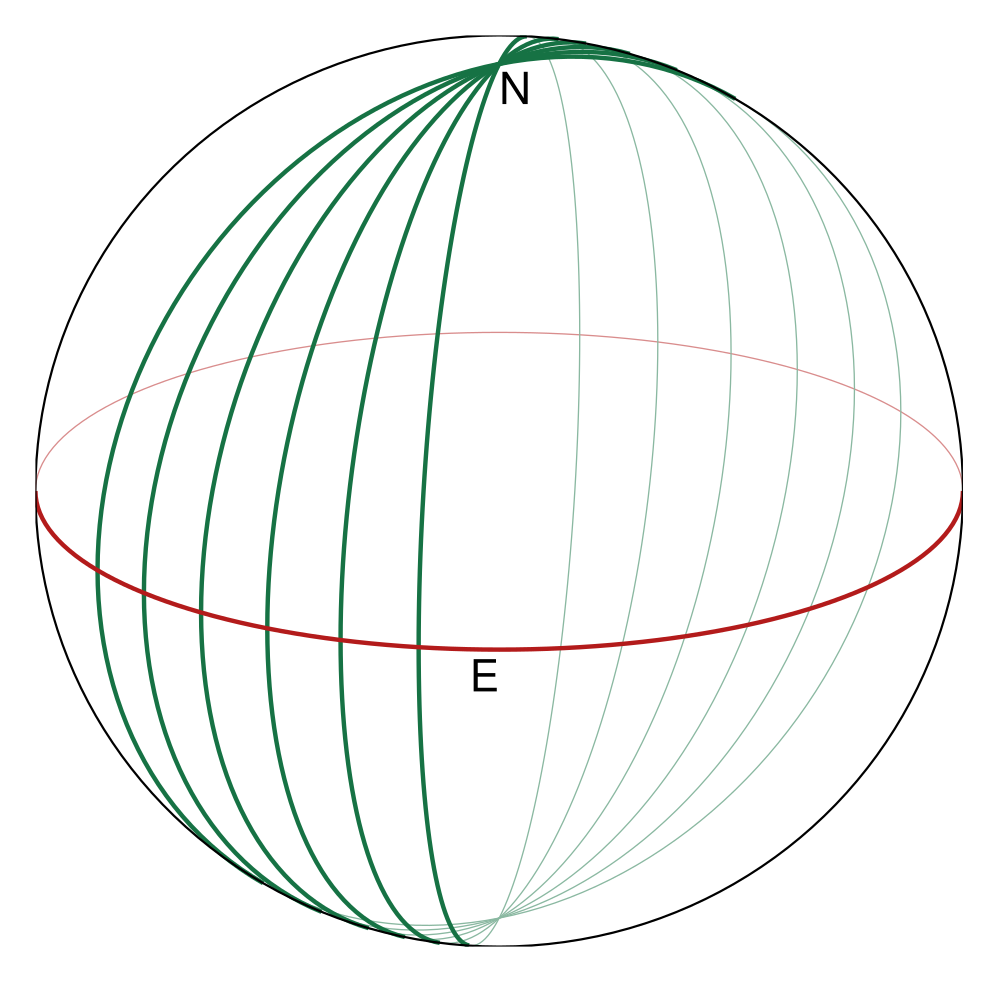
\includegraphics[width=0.65\textwidth]{~/Tesis/Figuras/A-Figuras/GeodesicasEsfera.png}
		\end{subfigure}
    \caption{Representación de algunas geodésicas en $\mathbb{R}^{2}$ y $\mathbb{S}^{2}$.}
	\end{figure}
\end{center}
